% defer/hazptr.tex
% Can I hazptr cheezeberger?

\section{Hazard Pointers}
\label{sec:defer:Hazard Pointers}

동시적으로 수행되는 레퍼런스 카운팅에서의 문제를 해결하는 한가지 방법은
레퍼런스 카운터들을 뒤집어서 구현하는 것으로,
데이터 원소에 저장되어 있는 정수를 증가시키는 게 아니라, CPU 별 (또는 쓰레드별)
리스트들에 그 데이터 원소로의 포인터를 저장해 두는 것입니다.
이런 리스트의 각 원소들은 \emph{해저드 포인터}~\cite{MagedMichael04a} 라고
불립니다.\footnote{
	그와 독립적으로 다른 사람들에 의해 개발된 것도
	있습니다~\cite{HerlihyLM02}.}
주어진 데이터 원소의 ``가상 레퍼런스 카운터'' 의 값은 그 원소를 레퍼런스 하고
있는 해저드 포인터들의 갯수를 세는 것으로 얻어질 수 있습니다.
따라서, 그 원소가 읽기를 하는 쓰레드들에 의해 접근할 수 없게 된다면, 그리고
더이상 그 원소를 레퍼런스 하고 있는 해저드 포인터가 더이상 존재하지 않는다면,
그 원소는 안전하게 메모리 해제될 수 있습니다.
\iffalse

One way of avoiding problems with concurrent reference counting
is to implement the reference counters
inside out, that is, rather than incrementing an integer stored in the
data element, instead store a pointer to that data element in
per-CPU (or per-thread) lists.
Each element of these lists is called a
\emph{hazard pointer}~\cite{MagedMichael04a}.\footnote{
	Also independently invented by others~\cite{HerlihyLM02}.}
The value of a given data element's ``virtual reference counter'' can
then be obtained by counting the number of hazard pointers referencing
that element.
Therefore, if that element has been rendered inaccessible to readers,
and there are no longer any hazard pointers referencing it, that element
may safely be freed.
\fi

{ \scriptsize
\begin{verbbox}
 1 int hp_store(void **p, void **hp)
 2 {
 3   void *tmp;
 4 
 5   tmp = ACCESS_ONCE(*p);
 6   ACCESS_ONCE(*hp) = tmp;
 7   smp_mb();
 8   if (tmp != ACCESS_ONCE(*p) ||
 9       tmp == HAZPTR_POISON) {
10     ACCESS_ONCE(*hp) = NULL;
11     return 0;
12   }
13   return 1;
14 }
15 
16 void hp_erase(void **hp)
17 {
18   smp_mb();
19   ACCESS_ONCE(*hp) = NULL;
20   hp_free(hp);
21 }
\end{verbbox}
}
\begin{figure}[tbp]
\centering
\theverbbox
\caption{Hazard-Pointer Storage and Erasure}
\label{fig:defer:Hazard-Pointer Storage and Erasure}
\end{figure}

물론, 이 말은 해저드 포인터 획득은 동시의 삭제들에 의한 정리 과정의 경주들을
막기 위해 매우 조심스럽게 행해져야만 합니다.
그런 한가지 구현이
Figure~\ref{fig:defer:Hazard-Pointer Storage and Erasure} 에 보여져 있는데,
line~1-13 에서 \co{hp_store()} 를 보이고 line~15-20 에서 \co{hp_erase()} 를
보이고 있습니다.
\co{smp_mb()} 기능은 Section~\ref{sec:advsync:Memory Barriers} 에서 자세히
설명될 겁니다만, 이 간단한 개략적 설명의 목표를 위해서는 무시되어도 될 겁니다.

\co{hp_store()} 함수는 동시의 수정을 체크하면서 \co{p} 에 의해 레퍼런스되는
포인터가 있는 데이터 원소를 위한 해저드 포인터를 \co{hp} 에 저장합니다.
동시의 수정이 이뤄졌다면, \co{hp_store()} 는 해저드 포인터를 저장하는 것을
거부하고 0을 리턴함으로써 호출자는 다시 처음부터 데이터 접근을 다시 시작해야
함을 알립니다.
그렇지 않다면, \co{hp_store()} 는 해당 데이터 원소를 위한 해저드 포인터를
성공적으로 기록했음을 알리기 위해 1을 리턴합니다.
\iffalse

Of course, this means that hazard-pointer acquisition must be carried
out quite carefully in order to avoid destructive races with concurrent
deletion.
One implementation is shown in
Figure~\ref{fig:defer:Hazard-Pointer Storage and Erasure},
which shows \co{hp_store()} on lines~1-13 and \co{hp_erase()} on
lines~15-20.
The \co{smp_mb()} primitive will be described in detail in
Section~\ref{sec:advsync:Memory Barriers}, but may be ignored for
the purposes of this brief overview.

The \co{hp_store()} function records a hazard pointer at \co{hp} for the data
element whose pointer is referenced by \co{p}, while checking for
concurrent modifications.
If a concurrent modification occurred, \co{hp_store()} refuses to record
a hazard pointer, and returns zero to indicate that the caller must
restart its traversal from the beginning.
Otherwise, \co{hp_store()} returns one to indicate that it successfully
recorded a hazard pointer for the data element.
\fi

\QuickQuiz{}
	Figure~\ref{fig:defer:Hazard-Pointer Storage and Erasure}
	의 \co{hp_store()} 는 왜 데이터 원소로의 접근을 두번이나 간접적으로
	하는거죠?
	왜 \co{void *} 가 아니라 \co{void **} 인 건가요?
	\iffalse

	Why does \co{hp_store()} in
	Figure~\ref{fig:defer:Hazard-Pointer Storage and Erasure}
	take a double indirection to the data element?
	Why not \co{void *} instead of \co{void **}?
	\fi
\QuickQuizAnswer{
	\co{hp_record()} 는 동시의 수정에 대해서 체크를 해봐야 하기 때문입니다.
	이 일을 하기 위해서는 그 원소로의 포인터로의 포인터가 필요한데, 그게
	있으면 해당 원소로의 포인터로의 수정이 있었는지 검사할 수 있기
	때문입니다.
	\iffalse

	Because \co{hp_record()} must check for concurrent modifications.
	To do that job, it needs a pointer to a pointer to the element,
	so that it can check for a modification to the pointer to the
	element.
	\fi
} \QuickQuizEnd

\QuickQuiz{}
	\co{hp_store()} 의 호출자는 실패했을 때 왜 데이터 접근을 처음부터 다시
	시작해야 하는거죠?
	데이터 구조체가 매우 크다면 좀 비효율적이지 않나요?
	\iffalse

	Why does \co{hp_store()}'s caller need to restart its
	traversal from the beginning in case of failure?
	Isn't that inefficient for large data structures?
	\fi
\QuickQuizAnswer{
	어떻게 보면 좀 비효율적일 수도 있겠습니다만 분명한 사실은 정확성을 위해
	그런 처음부터의 재시작이 반드시 필요하다는 점입니다.
	이를 확실히 보기 위해, 원소~A, B, 그리고~C 를 가지고 있는 해저드
	포인터로 보호되는 링크드 리스트가 다음의 일련의 이벤트들을 받는다고
	생각해 봅시다:
	\iffalse

	It might be inefficient in some sense, but the fact is that
	such restarting is absolutely required for correctness.
	To see this, consider a hazard-pointer-protected linked list
	containing elements~A, B, and~C that is subjecte to the
	following sequence of events:
	\fi

	\begin{enumerate}
	\item	쓰레드~0 가 원소~B 로의 해저드 포인터를 저장합니다
		(아마도 원소~A 를 거쳐 원소~B 를 찾아왔을 겁니다).
	\item	쓰레드~1 이 리스트로부터 원소~B 를 삭제하는데, 이를 위해 원소~B
		에서 원소~C 로의 포인터를 이 삭제 작업을 표시하기 위해 특수한
		\co{HAZPTR_POISON} 값으로 설정합니다.
		Thread~0 는 원소~B 로의 해저드 포인터를 가지고 있으므로, 아직
		정리될 수 없습니다.
	\item	쓰레드~1 이 리스트에서 원소~C 를 삭제합니다.
		원소~C 를 레퍼런스 하는 해저드 포인터들이 존재하지 않으므로,
		원소~C 는 곧바로 메모리 해제될 수 있습니다.
	\item	쓰레드~0 이 이제 없어진 원소~B 의 다음 원소로의 해저드 포인터를
		얻으려 합니다만, \co{HAZPTR_POISON} 값을 보게 되고, 따라서 0을
		리턴해서, 호출자가 리스트의 시작점부터 탐색을 다시 시작하도록
		강제합니다.
	\iffalse

	\item	Thread~0 stores a hazard pointer to element~B
		(having presumably traversed to element~B from element~A).
	\item	Thread~1 removes element~B from the list, which sets
		the pointer from element~B to element~C to a special
		\co{HAZPTR_POISON} value in order to mark the deletion.
		Because Thread~0 has a hazard pointer to element~B,
		it cannot yet be freed.
	\item	Thread~1 removes element~C from the list.
		Because there are no hazard pointers referencing element~C,
		it is immediately freed.
	\item	Thread~0 attempts to acquire a hazard pointer to
		now-removed element~B's successor, but sees the
		\co{HAZPTR_POISON} value, and thus returns zero,
		forcing the caller to restart its traversal from the
		beginning of the list.
	\fi
	\end{enumerate}

	따라서 처음부터 다시 탐색하는게 좋은 방법인데, 이렇게 하지 않는다면
	쓰레드~0 는 이제는 제거된 원소~C 에 액세스를 시도할 수 있는데, 이는
	임의의 끔찍한 메모리 오염을 일으키는 결과를 만들어낼 수 있는데, 특히나
	원소~C 를 위해 사용되던 메모리가 어떤 다른 목적으로 재할당 되었다면
	특히 그럴 것이기 때문입니다.

	그와는 별개로, 해저드 포인터의 재시작은 최소한의 메모리 사용량을 유지할
	수 있도록 함을 이해하기 바랍니다.
	현재 해저드 포인터로 레퍼런스 되고 있지 않은 오브젝트는 곧바로 해제될
	수 있습니다.
	대조적으로,
	Section~\ref{sec:defer:Read-Copy Update (RCU)} 에서는 read-side
	재시도를 방지하지만 (read-side 오버헤드도 최소화 시킵니다), 훨씬 큰
	메모리 사용량을 갖는 메커니즘을 이야기할 겁니다.
	\iffalse

	Which is a very good thing, because otherwise Thread~0 would
	have attempted to access the now-freed element~C,
	which might have resulted in arbitrarily horrible
	memory corruption, especially if the memory for
	element~C had since been re-allocated for some other
	purpose.

	All that aside, please understand that hazard pointers's
	restarting allows it to maintain a minimal memory footprint.
	Any object not currently referenced by some hazard pointer
	may be immediately freed.
	In contrast,
	Section~\ref{sec:defer:Read-Copy Update (RCU)}
	will discuss a mechanism that avoids read-side retries
	(and minimizes read-side overhead), but has a much larger
	memory footprint.
	\fi
} \QuickQuizEnd

\QuickQuiz{}
	해저드 포인터들에 대한 논문들은 각각의 포인터의 아래 비트들을 지워진
	원소들을 마크하기 위해 사용한다고 하는데, \co{HAZPTR_POISON} 은 뭔가요?
	\iffalse

	Given that papers on hazard pointers use the bottom bits
	of each pointer to mark deleted elements, what is up with
	\co{HAZPTR_POISON}?
	\fi
\QuickQuizAnswer{
	출간된 논문의 해저드 포인터 구현들은 그 삽입과 삭제를 위해 non-blocking
	동기화 기법들을 사용했습니다.
	이런 기법들은 데이터 구조체를 가로지르며 읽기를 하는 쓰레드들이
	업데이트를 하는 쓰레드들이 그들의 업데이트를 완료하도록 ``도움''을 줄
	것을 필요로 하는데, 이 말은 읽기를 하는 쓰레드들은 삭제된 원소의 다음
	원소를 봐야만 한다는 뜻입니다.

	반면에, 우리는 업데이트 작업들을 동기화 시키는데 락킹을 사용할 것인데,
	이렇게 되면 읽기를 하는 쓰레드들이 업데이트를 하는 쓰레드들이 그들의
	업데이트를 완료할 수 있도록 돕는 일을 해줄 필요가 없어져서 포인터들의
	아래쪽 비트들을 놔둘 수 있게 해줍니다.
	이 방법은 읽기를 하는쪽 코드를 좀 더 간단하고 빠르게 해줍니다.
	\iffalse

	The published implementations of hazard pointers used
	non-blocking synchronization techniques for insertion
	and deletion.
	These techniques require that readers traversing the
	data structure ``help'' updaters complete their updates,
	which in turn means that readers need to look at the successor
	of a deleted element.

	In contrast, we will be using locking to synchronize updates,
	which does away with the need for readers to help updaters
	complete their updates, which in turn allows us to leave
	pointers' bottom bits alone.
	This approach allows read-side code to be simpler and faster.
	\fi
} \QuickQuizEnd

해저드 포인터들을 사용하는 알고리즘들은 데이터 구조체를 지나가는 중 어떤
단계에서든 재시작할 수 있으므로, 그런 알고리즘들은 모든 필요한 해저드
포인터들을 얻어오는 작업이 끝나기 전까지는 이 데이터 구조체에 어떤 변경을
가하지 않도록 특별한 주의를 반드시 기울여야만 합니다.
\iffalse

Because algorithms using hazard pointers might be restarted at any
step of their traversal through the data structure, such algorithms
must typically take care to avoid making any changes to the data
structure until after they have acquired all relevant hazard pointers.
\fi

\QuickQuiz{}
	하지만 해저드 포인터들에 있는 이런 제약사항들은 다른 형태의 레퍼런스
	카운팅에도 똑같이 적용되는 거 아닌가요?
	\iffalse

	But don't these restrictions on hazard pointers also apply
	to other forms of reference counting?
	\fi
\QuickQuizAnswer{
	이런 제약사항은 레퍼런스 획득이 실패할 수 있는 레퍼런스 카운팅
	메커니즘들에만 적용됩니다.
	\iffalse

	These restrictions apply only to reference-counting mechanisms whose
	reference acquisition can fail.
	\fi
} \QuickQuizEnd

이런 제약사항들은 읽기를 하는 쓰레드들에는 커다란 이득으로 귀결되는데, 해저드
포인터들은 각 CPU/쓰레드에 지역적으로 저장되기 때문으로, 이에 의해 데이터
구조체들을 횡단하는 작업은 완전히 읽기만 하면서 행해질 수 있다는 사실 덕입니다.
page~\pageref{fig:count:Optimization and the Four Parallel-Programming Tasks}
의
Figure~\ref{fig:count:Optimization and the Four Parallel-Programming Tasks}
를 다시 인용하자면, 해저드 포인터들은 CPU 캐시들이 리소스 복사를 할 수 있게
해서 병렬 액세스 컨트롤 메커니즘을 약화시키는 걸 가능하게 하고, 따라서 성능과
확장성을 높여줍니다.
다른 메커니즘들과의 성능 비교는 Chapter~\ref{chp:Data Structures} 와 다른
출간물들~\cite{ThomasEHart2007a,McKenney:2013:SDS:2483852.2483867,MagedMichael04a}
에서 얻을 수 있을 겁니다.

해저드 포인터들은 레퍼런스 카운터들보다 훨씬 더 확장성 있습니다만 여전히 읽기를
하는 쓰레드들이 공유 메모리에 쓰기를 하게 합니다.
다음 섹션의 주제인 시퀀스 카운터들은 읽기 쪽의 쓰기를 완전히 막습니다.
\iffalse

These restrictions result in great benefits to readers, courtesy of the
fact that the hazard pointers are stored local to each CPU/thread,
which in turn allows traversals of the data structures themselves to
be carried out in a completely read-only fashion.
Referring back to
Figure~\ref{fig:count:Optimization and the Four Parallel-Programming Tasks}
on
page~\pageref{fig:count:Optimization and the Four Parallel-Programming Tasks},
hazard pointers enable the CPU caches to do resource replication, which
in turn allows weakening of the parallel-access-control mechanism,
thus boosting performance and scalability.
Performance comparisons with other mechanisms may be found in
Chapter~\ref{chp:Data Structures}
and in other publications~\cite{ThomasEHart2007a,McKenney:2013:SDS:2483852.2483867,MagedMichael04a}.
\fi

{ \scriptsize
\begin{verbbox}
 1 struct route_entry {
 2   struct hazptr_head hh;
 3   struct route_entry *re_next;
 4   unsigned long addr;
 5   unsigned long iface;
 6   int re_freed;
 7 };
 8 struct route_entry route_list;
 9 DEFINE_SPINLOCK(routelock);
10 hazard_pointer __thread *my_hazptr;
11
12 unsigned long route_lookup(unsigned long addr)
13 {
14   int offset = 0;
15   struct route_entry *rep;
16   struct route_entry **repp;
17
18 retry:
19   repp = &route_list.re_next;
20   do {
21     rep = ACCESS_ONCE(*repp);
22     if (rep == NULL)
23       return ULONG_MAX;
24     if (rep == (struct route_entry *)HAZPTR_POISON)
25       goto retry;
26     my_hazptr[offset].p = &rep->hh;
27     offset = !offset;
28     smp_mb();
29     if (ACCESS_ONCE(*repp) != rep)
30       goto retry;
31     repp = &rep->re_next;
32   } while (rep->addr != addr);
33   if (ACCESS_ONCE(rep->re_freed))
34     abort();
35   return rep->iface;
36 }
\end{verbbox}
}
\begin{figure}[bp]
\centering
\theverbbox
\caption{Hazard-Pointer Pre-BSD Routing Table Lookup}
\label{fig:defer:Hazard-Pointer Pre-BSD Routing Table Lookup}
\end{figure}

{ \scriptsize
\begin{verbbox}
 1 int route_add(unsigned long addr,
 2               unsigned long interface)
 3 {
 4   struct route_entry *rep;
 5
 6   rep = malloc(sizeof(*rep));
 7   if (!rep)
 8     return -ENOMEM;
 9   rep->addr = addr;
10   rep->iface = interface;
11   rep->re_freed = 0;
12   spin_lock(&routelock);
13   rep->re_next = route_list.re_next;
14   route_list.re_next = rep;
15   spin_unlock(&routelock);
16   return 0;
17 }
18
19 int route_del(unsigned long addr)
20 {
21   struct route_entry *rep;
22   struct route_entry **repp;
23
24   spin_lock(&routelock);
25   repp = &route_list.re_next;
26   for (;;) {
27     rep = *repp;
28     if (rep == NULL)
29       break;
30     if (rep->addr == addr) {
31       *repp = rep->re_next;
32       rep->re_next =
33           (struct route_entry *)HAZPTR_POISON;
34       spin_unlock(&routelock);
35       hazptr_free_later(&rep->hh);
36       return 0;
37     }
38     repp = &rep->re_next;
39   }
40   spin_unlock(&routelock);
41   return -ENOENT;
42 }
\end{verbbox}
}
\begin{figure}[bp]
\centering
\theverbbox
\caption{Hazard-Pointer Pre-BSD Routing Table Add/Delete}
\label{fig:defer:Hazard-Pointer Pre-BSD Routing Table Add/Delete}
\end{figure}

The Pre-BSD routing example can use hazard pointers as shown in
Figure~\ref{fig:defer:Hazard-Pointer Pre-BSD Routing Table Lookup}
for data structures and \co{route_lookup()}, and in
Figure~\ref{fig:defer:Hazard-Pointer Pre-BSD Routing Table Add/Delete}
for \co{route_add()} and \co{route_del()}
(\path{route_hazptr.c}).
As with reference counting, the hazard-pointers implementation
is quite similar to the sequential algorithm shown in
Figure~\ref{fig:defer:Sequential Pre-BSD Routing Table}
on
page~\pageref{fig:defer:Sequential Pre-BSD Routing Table},
so only differences will be discussed.

Starting with
Figure~\ref{fig:defer:Hazard-Pointer Pre-BSD Routing Table Lookup},
line~2 shows the \co{->hh} field used to queue objects pending
hazard-pointer free,
line~6 shows the \co{->re_freed} field used to detect use-after-free bugs,
and lines~24-30 attempt to acquire a hazard pointer, branching
to line~18's \co{retry} label on failure.

In
Figure~\ref{fig:defer:Hazard-Pointer Pre-BSD Routing Table Add/Delete},
line~11 initializes \co{->re_freed},
lines~32 and~33 poison the \co{->re_next} field of the newly removed
object, and
line~35 passes that object to the hazard pointers's
\co{hazptr_free_later()} function, which will free that object once it
is safe to do so.
The spinlocks work the same as in
Figure~\ref{fig:defer:Reference-Counted Pre-BSD Routing Table Add/Delete}.

\begin{figure}[tb]
\centering
\resizebox{2.5in}{!}{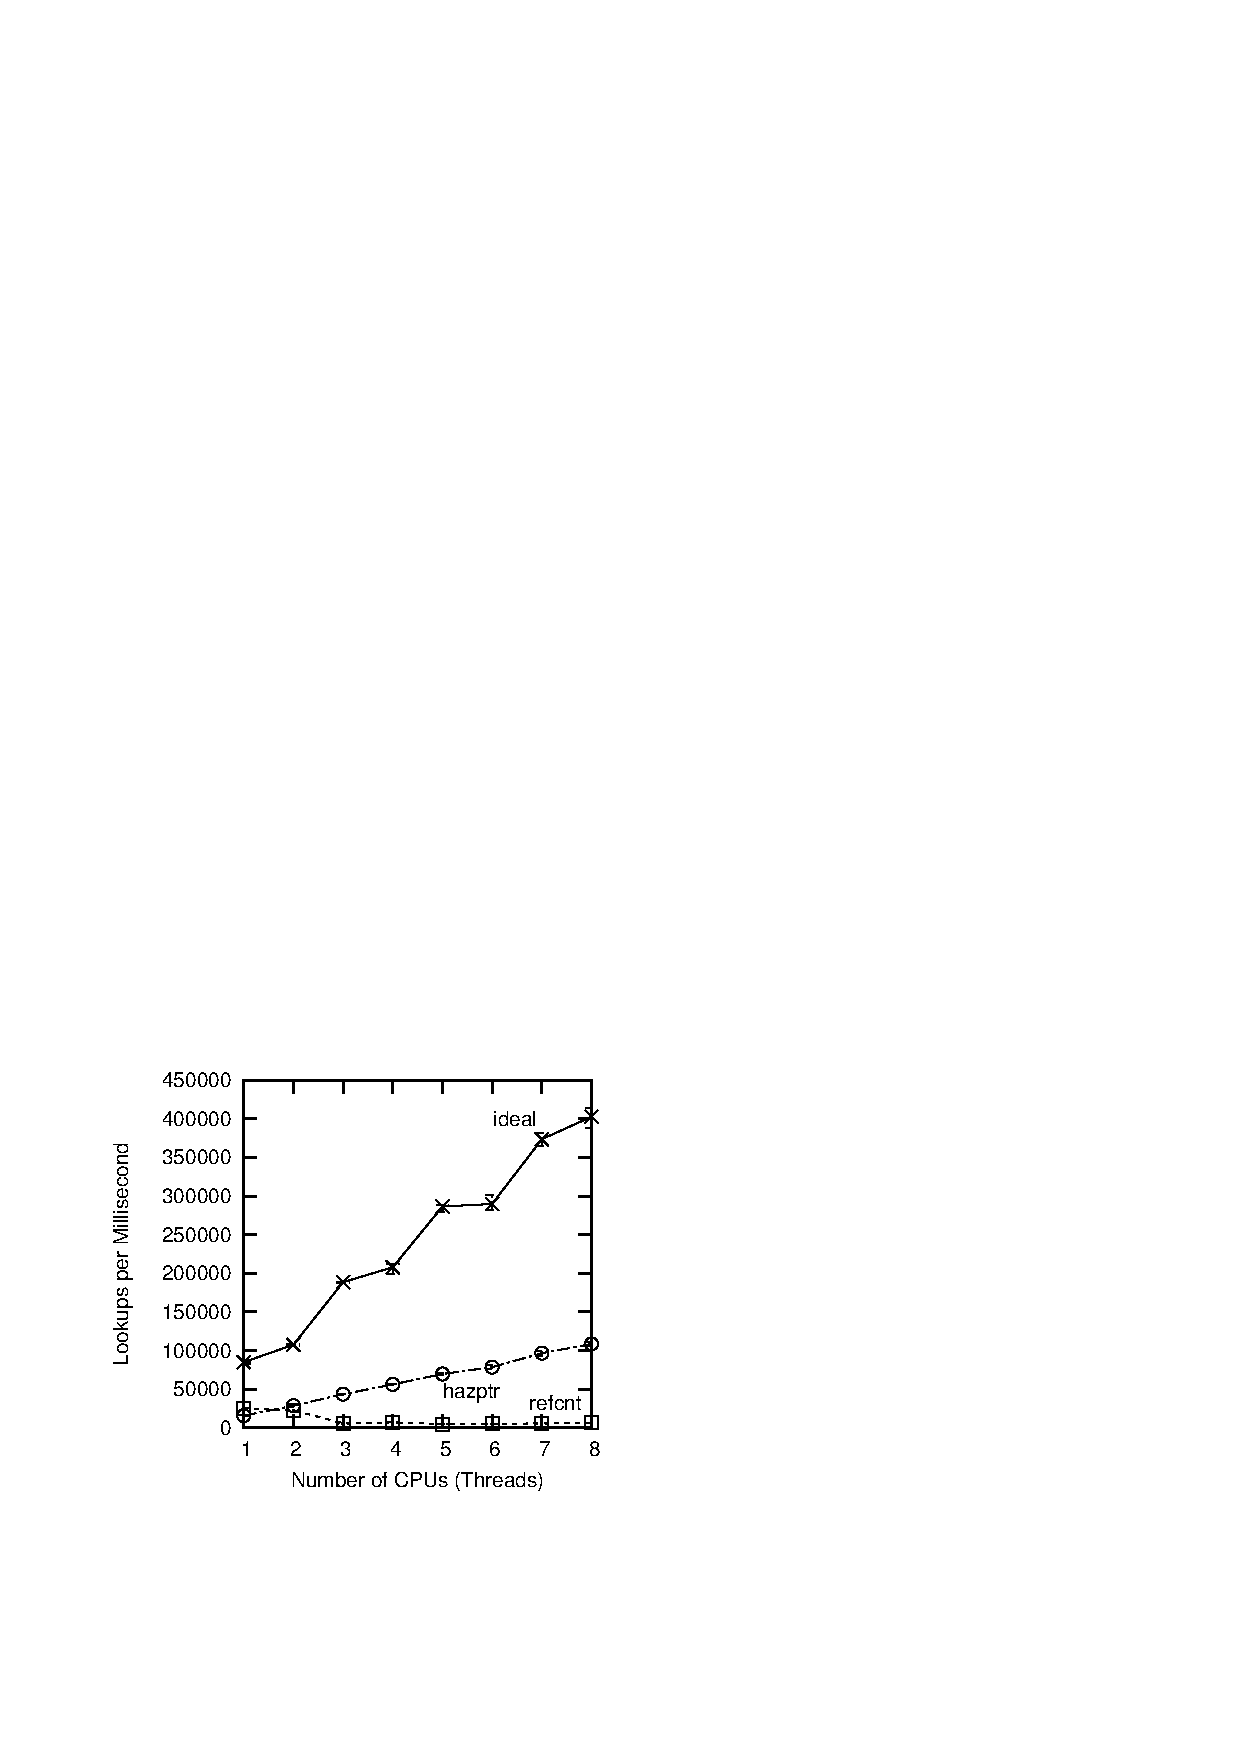
\includegraphics{CodeSamples/defer/data/paulmck.2016/perf-hazptr}}
\caption{Pre-BSD Routing Table Protected by Hazard Pointers}
\label{fig:defer:Pre-BSD Routing Table Protected by Hazard Pointers}
\end{figure}

Figure~\ref{fig:defer:Pre-BSD Routing Table Protected by Hazard Pointers}
shows the hazard-pointers-protected Pre-BSD routing algorithm's
performance on the same read-only workload as for
Figure~\ref{fig:defer:Pre-BSD Routing Table Protected by Reference Counting}.
Although hazard pointers scales much better than does reference counting,
hazard pointers still require readers to do writes to shared
memory (albeit with much improved locality of reference),
and also require a full memory barrier and retry check for each
object traversed.
Therefore, hazard pointers's performance is far short of ideal.
On the other hand, hazard pointers do operate correctly for workloads
involving concurrent updates.

\QuickQuiz{}
	The paper ``Structured Deferral: Synchronization via
	Procrastination''~\cite{McKenney:2013:SDS:2483852.2483867}
	shows that hazard pointers have near-ideal performance.
	Whatever happened in
	Figure~\ref{fig:defer:Pre-BSD Routing Table Protected by Hazard Pointers}???
\QuickQuizAnswer{
	First,
	Figure~\ref{fig:defer:Pre-BSD Routing Table Protected by Hazard Pointers}
	has a linear y-axis, while most of the graphs in the
	``Structured Deferral'' paper have logscale y-axes.
	Next, that paper uses hash tables, while
	Figure~\ref{fig:defer:Pre-BSD Routing Table Protected by Hazard Pointers}'s
	uses a simple linked list.
	Finally, that paper used a larger and older x86 system, while
	a newer but smaller system that was used to generate the data
	shown in
	Figure~\ref{fig:defer:Pre-BSD Routing Table Protected by Hazard Pointers}.
} \QuickQuizEnd

The next section attempts to improve on hazard pointers by using
sequence locks, which avoid both read-side writes and per-object memory
barriers.
